% Draft for ICML 2027. Swap \documentclass/usepackage for the official icml2027 style when released.
\documentclass[10pt]{article}
\usepackage[margin=1in]{geometry}
\usepackage{amsmath,amssymb,amsthm,booktabs,graphicx,hyperref,xcolor}
\newtheorem{proposition}{Proposition}
\newtheorem{definition}{Definition}
\newcommand{\todo}[1]{\textcolor{red}{[TODO: #1]}}
\newcommand{\Unk}{\textsc{Unknown}}

\title{Who Wrote What Survived? Edit-Factorized Provenance with Certified Abstention for Human--AI Co-Written Text}
\author{Anonymous}
\date{}

\begin{document}
\maketitle

\begin{abstract}
AI-text detectors return a single score per document. Most text, however, is now co-written: humans draft and AI polishes, or AI drafts and humans edit, often over several rounds. We show that such a score is not a measure of contribution. Among AI-edited documents of the EditLens benchmark, zero-shot detector scores correlate only weakly with the true fraction of AI-written words (Spearman $\rho\!\approx\!0.2$). Within a single score decile, that fraction spans $0.66$ (10th--90th percentile). Contribution is itself ill-posed without a stated attribution policy: under two defensible policies, the AI share of the same lightly polished document differs by $48$ points on average.

We therefore recast detection as \emph{retained provenance}. Each word of the final text is labelled with the author of the last edit that wrote it, under an explicit policy, and the model abstains where the evidence cannot decide. We prove that text-only provenance is non-identifiable and bound the coverage any detector can reach at a target error rate.

We then propose \textbf{ProvSeg}, which models the recursive definition of provenance directly: a word's author is the editor if it was edited and is inherited from the base otherwise. This gives $P(A)=\pi\rho+(1-\pi)\beta$, where $\pi$ is the probability that the word was edited, $\rho$ that the editor is AI, and $\beta$ that the base author is AI. We show that in the human-draft/AI-polish regime, word provenance is \emph{exactly as hard as edit detection}. Each factor is an additive bottleneck over named evidence channels (LLM likelihood, hidden representation, context, dependency syntax), so every decision comes with an exact \emph{history explanation}, and the uncertainty splits exactly into edit-, editor- and base-uncertainty. Version pairs supervise $\pi$ during training only, and Learn-then-Test turns uncertainty into a certified \Unk. \todo{headline results on 7 benchmarks}.
\end{abstract}

\section{Introduction}
\todo{Teaser Fig.~1: accuracy vs.\ polish degree; baselines degrade, ProvSeg+abstain stays accurate with shrinking coverage and names the conflicting evidence.}

\paragraph{A score is not a contribution (Fig.~\ref{fig:m1}).}
EditLens~\cite{editlens} releases human, AI-edited and AI-generated documents together with the source text, which lets us compute the true fraction of AI-written words by alignment. Its document scores give the following picture:
\begin{itemize}
\item Binoculars and Fast-DetectGPT reach $\rho=0.68/0.69$ over all documents, but only $\rho=0.22/0.21$ among AI-edited ones, which is exactly the co-writing regime.
\item Within one score decile, the true AI fraction ranges over $0.66$.
\item Even supervised detectors (EditLens, Pangram) leave a $0.38$--$0.42$ range.
\end{itemize}
A teacher who reads ``87\% AI'' cannot tell 20\% from 80\% of the words.

\paragraph{Contribution needs a policy (Fig.~\ref{fig:m2}).}
On version-paired data (APT-Eval, Beemo), we compare a word-level retained policy with a sentence-level policy, in which any sentence the editor touched belongs to the editor. The two policies disagree on $44$--$62\%$ of the words of polished documents. The document AI share moves by $48$ points on average at the \emph{lightest} polish level ($80$ points at the 90th percentile). The question ``how much did AI write?'' has no answer until \emph{where} and \emph{under which policy} are fixed.

\paragraph{Contributions.}
\begin{enumerate}
\item \textbf{Problem and evidence of need.} Retained word-level provenance with an explicit policy, and two measurement studies showing that document scores are not contributions.
\item \textbf{Theory.} Non-identifiability, a coverage ceiling $c\le\frac{1/2-\varepsilon}{1/2-\alpha}$, and a proof that version records can only help.
\item \textbf{Edit-Factorized Provenance.} A model that mirrors the recursive definition of provenance, $P(A)=\pi\rho+(1-\pi)\beta$. An exact error decomposition (Prop.~\ref{prop:dec}) and a reduction theorem show that provenance is as hard as edit detection whenever authors are distinguishable (Prop.~\ref{prop:red}).
\item \textbf{History explanations with exact evidence.} Each factor is an additive bottleneck over named evidence channels: LLM likelihood, RepreGuard-style representation, context, and PRDetect-style dependency syntax. A span is explained as ``edited ($\pi$) by an AI-like editor ($\rho$) over a human base ($\beta$)'', with the channel that decides each factor.
\item \textbf{Privileged versions and certified, explained abstention.} Version pairs supervise $\pi$ during training only, and observed versions plug in exactly at test time (records track). The predictive variance splits into edit-, editor- and base-uncertainty, so each certified \Unk{} states its cause.
\end{enumerate}

\section{Related Work}
Document detectors: DetectGPT, Fast-DetectGPT, Binoculars, RepreGuard, PRDetect; benchmarks RAID, DetectRL. Fine-grained/mixed: SeqXGPT, PASTED, SemEval-24 8C/M4GT-Bench, HACo-Det, SenDetEX, EditLens, Beemo, APT-Eval. Explanations for detectors: post-hoc saliency, LLM rationales, retrieval-based exemplars (ExaGPT). Self-explaining models: concept bottlenecks, neural additive models; learning with privileged information; heteroscedastic uncertainty; Learn-then-Test and conformal risk control. \todo{verify 2026 preprints}

\section{Retained Provenance and Its Limits}
\begin{definition}[Retained provenance]
A history $h=((v_0,a_0),\dots,(v_K,a_K))$ consists of versions $v_k$ with authors $a_k\in\{H,A\}$, and $x=v_K$ is the final text. The label $y_i(h)$ of word $x_i$ is $a_k$ for the largest $k$ such that $x_i$ is not copied from $v_{k-1}$. The edit indicator $e_i(h)=1$ iff $x_i$ is not copied from $v_{K-1}$.
\end{definition}
Let $\eta_i(x)=P(y_i=A\mid x)$ and $\varepsilon=\mathbb{E}_{x,i}\min(\eta_i,1-\eta_i)$.

\begin{proposition}[Non-identifiability]\label{prop:nonid}
If with positive probability distinct histories with the same final text disagree on $y_i$, then $\varepsilon>0$, and every full-coverage text-only tagger errs on at least a fraction $\varepsilon$ of words.
\end{proposition}

\begin{proposition}[Coverage ceiling]\label{prop:cov}
For $\alpha<\tfrac12$, any text-only selective tagger with selective risk at most $\alpha$ has coverage $c\le\frac{1/2-\varepsilon}{1/2-\alpha}$.
\end{proposition}
\begin{proof}
Let $S$ be the set of answered words. On $S$ the error is at least $\mathbb{E}[\min(\eta,1-\eta)\mid S]$ and at most $\alpha$. Off $S$, $\min(\eta,1-\eta)\le\tfrac12$. Hence $\varepsilon\le c\alpha+(1-c)/2$.
\end{proof}

\begin{proposition}[Records cannot hurt]\label{prop:records}
For any record $r$ (earlier versions or logs), $\varepsilon(x,r)\le\varepsilon(x)$.
\end{proposition}
\begin{proof}
$t\mapsto\min(t,1-t)$ is concave, and $\eta(x)=\mathbb{E}[\eta(x,r)\mid x]$. Apply Jensen's inequality.
\end{proof}

\section{ProvSeg: Edit-Factorized Provenance}
\paragraph{From the definition to the model.} Retained provenance is recursive: $y_i=a_K$ if $e_i=1$, and $y_i=y_i^{(K-1)}$ otherwise. ProvSeg models this structure directly instead of training a flat classifier:
\begin{equation}
P(y_i{=}A\mid x)=\pi_i\rho_i+(1-\pi_i)\beta_i,
\label{eq:efp}
\end{equation}
\begin{itemize}
\item $\pi_i=P(e_i{=}1\mid x)$: was the word written in the last edit?
\item $\rho_i=P(a_K{=}A\mid x,e_i{=}1)$: who made that edit?
\item $\beta_i=P(y^{(K-1)}_i{=}A\mid x,e_i{=}0)$: who wrote the retained base?
\end{itemize}

\begin{proposition}[Exact error decomposition]\label{prop:dec}
For any estimates $\hat\pi,\hat\rho,\hat\beta$ and $\hat p=\hat\pi\hat\rho+(1-\hat\pi)\hat\beta$,
\[\hat p-p=(\hat\pi-\pi)(\rho-\beta)+\hat\pi(\hat\rho-\rho)+(1-\hat\pi)(\hat\beta-\beta).\]
\end{proposition}
\noindent The identity follows by adding and subtracting $\hat\pi\rho$ and $(1-\hat\pi)\beta$. It shows that edit-detection errors are harmful \emph{only where editor and base differ}, i.e.\ where $|\rho-\beta|$ is large. Privileged edit supervision targets exactly the first term.

\begin{proposition}[Provenance reduces to edit detection]\label{prop:red}
Suppose the editor and the base author are identifiable from $x$, i.e.\ $\rho_i,\beta_i\in\{0,1\}$ with $\rho_i\neq\beta_i$. Then the word-level Bayes error of provenance equals the Bayes error of edit detection, $\mathbb{E}\min(\pi,1-\pi)$. If instead $\rho_i=\beta_i$, provenance does not depend on $e_i$, and the Bayes error is $\mathbb{E}\min(\rho,1-\rho)$.
\end{proposition}
\noindent In the human-draft/AI-polish regime, this proposition states that \emph{who wrote a word} is exactly as hard as \emph{whether it was touched}. The polish-degree curve (Fig.~1) therefore measures edit detectability, and observing $e$ (the records track) removes this term entirely.

\paragraph{Evidence channels and exact factor explanations.} Five named channels produce per-word states $h_k(i)$:
\begin{itemize}
\item LLM-likelihood: observer/performer log-probabilities, entropy, Binoculars cross-entropy, Fast-DetectGPT $z$, and GLTR rank;
\item hidden representation: a RepreGuard-style projection;
\item context: DeBERTa-v3 word states;
\item dependency syntax: a 2-layer GCN over the spaCy tree, i.e.\ the PRDetect graph applied per word.
\end{itemize}
Each factor $f\in\{\pi,\rho,\beta\}$ is an additive bottleneck, $\mathrm{logit}\,f_i=b_f+\sum_k v_{f,k}^\top h_k(i)$. The explanation of a span is therefore a \emph{history}: whether it was edited, by whom, and over what base, with the evidence channel that decides each factor. Within each factor the attribution is exact. Channel dropout ($p=0.1$) keeps every channel informative on its own.

\paragraph{Uncertainty with a cause.} By the law of total variance,
\[p(1-p)=\underbrace{\pi(1-\pi)(\rho-\beta)^2}_{\text{edit-uncertain}}+\underbrace{\pi\rho(1-\rho)}_{\text{editor-uncertain}}+\underbrace{(1-\pi)\beta(1-\beta)}_{\text{base-uncertain}}.\]
Every \Unk{} span therefore reports which of the three sources caused it. Abstention uses CRF marginals with a Learn-then-Test threshold (fixed-sequence, Hoeffding--Bentkus) on calibration documents, which gives $P(R(\hat\lambda)\le\alpha)\ge1-\delta$.

\paragraph{Training with privileged versions.} The emissions are $\pm\frac12\mathrm{logit}\,p_i$, fed to a linear-chain CRF. The loss is
\[\mathcal{L}=\mathrm{NLL}_{\mathrm{CRF}}+\lambda_e\mathrm{BCE}(\pi,e)+\lambda_f\big[\mathrm{BCE}(\rho,y)\,|_{e=1}+\mathrm{BCE}(\beta,y)\,|_{e=0}\big],\]
where $e$ is available only for version-paired training data (Beemo, PASTED, EditLens-val). On SeqXGPT and SemEval, $\pi$ is a latent variable learned through the CRF term. At test time only $x$ is used. The \emph{records track} plugs the observed $e$ into Eq.~\eqref{eq:efp}, which by Prop.~\ref{prop:records} cannot increase Bayes error.

\section{Experiments}
\paragraph{Data.} The training set consists of the train splits of SeqXGPT-Bench, SemEval-24 8C, Beemo, PASTED and EditLens-val (25k documents per set at most). Held-out sets are PASTED-OOD (unseen paraphraser), APT-Eval (unseen polishers, graded degrees) and EditLens-test.
\paragraph{Baselines.} Binoculars$^*$, Fast-DetectGPT$^*$, log-likelihood$^*$ and RepreGuard$^*$, adapted to word level with a sliding window and a dev-optimal Platt calibration. Trained baselines: Seq-RoBERTa (CRF) and a SeqXGPT-style feature tagger. Ablations: black box (no bottleneck), no syntax, no edit supervision, no ambiguity head, no LLM features.
\todo{Table 1 accuracy; Table 2 selective coverage at $\alpha$ and validity; Table 3 explanation (deletion/sufficiency, edit AUROC, ambiguity--error AUROC, channel shares by edit type); Fig.~2 risk--coverage; Fig.~3 validity; case studies.}

\begin{figure}[t]\centering
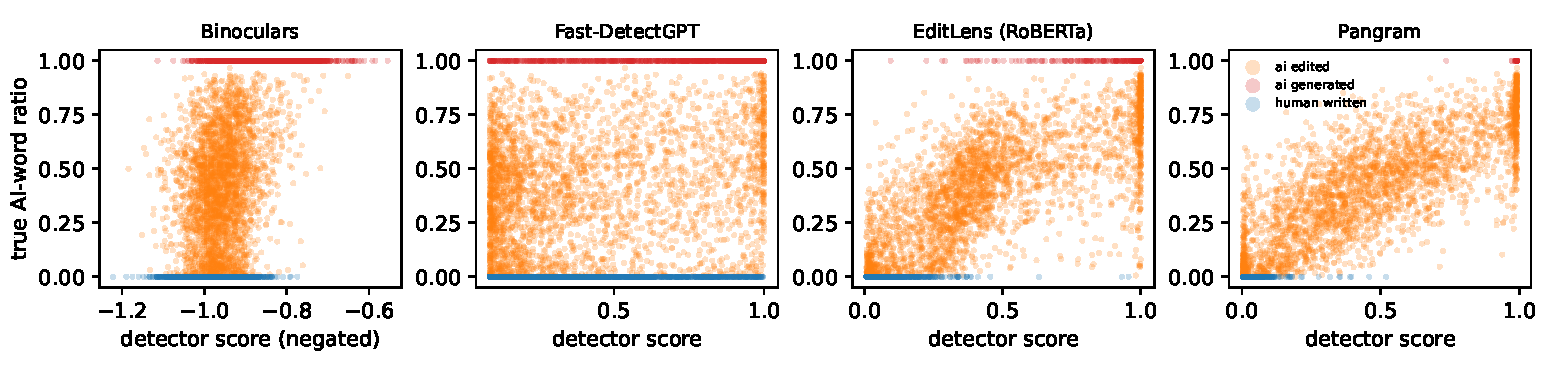
\includegraphics[width=\linewidth]{figs/figM1_score_vs_ratio.pdf}
\caption{Document detector scores vs.\ the true fraction of AI-written words on EditLens. AI-edited documents (orange) are spread over the whole range of scores.}\label{fig:m1}
\end{figure}
\begin{figure}[t]\centering
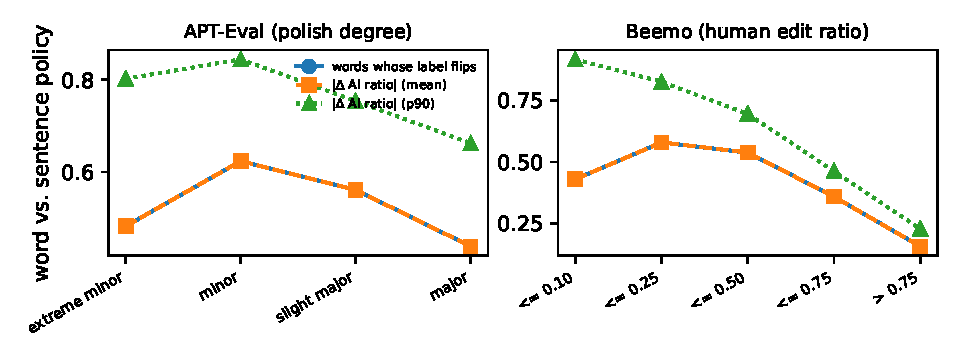
\includegraphics[width=.8\linewidth]{figs/figM2_policy.pdf}
\caption{The same documents under word-level and sentence-level attribution policies: fraction of words whose label flips, and the gap in AI share.}\label{fig:m2}
\end{figure}

\section{Limitations}
Labels describe surviving wording, not ideas or effort. Diff alignment may over-attribute copied function words. The guarantee requires exchangeable calibration documents (we report OOD validity separately). Channels are informative but not causal claims about authorship. The study covers English only.

\bibliographystyle{plain}
\begin{thebibliography}{9}
\bibitem{editlens} Pangram Labs. EditLens. ICLR 2026.
\end{thebibliography}
\end{document}
